%"The PDF file may contain up to 25 pages of reference material, single-sided, letter or A4 size, with text and illustrations readable by a person with correctable eyesight without magnification from a distance of 1/2 meter."
\documentclass[10pt,landscape,twocolumn,a4paper,notitlepage]{article}
\usepackage{hyperref}
\usepackage[english, activeacute]{babel}
\usepackage[utf8]{inputenc}
\usepackage{fancyhdr}
\usepackage{lastpage}
\usepackage{listings}
\usepackage{amssymb}
\usepackage[usenames,dvipsnames]{color}
\usepackage{graphicx}
\usepackage{wrapfig}
\usepackage{amsmath}
\usepackage{makeidx}

%%% Margenes
\setlength{\columnsep}{0.25in}    % default=10pt
\setlength{\columnseprule}{0.5pt}    % default=0pt (no line)

\addtolength{\textheight}{2.35in}
\addtolength{\topmargin}{-0.9in}     % ~ -0.5 del incremento anterior

\addtolength{\textwidth}{1.1in}
\addtolength{\oddsidemargin}{-0.55in} % -0.5 del incremento anterior

\setlength{\headsep}{0.08in}
\setlength{\parskip}{0in}
\setlength{\headheight}{15pt}
\setlength{\parindent}{0mm}

%%% Encabezado y pie de pagina
\pagestyle{fancy}
\fancyhead[LO]{\textbf{\title}}
\fancyhead[C]{\leftmark\ -\ \rightmark}
\fancyhead[RO]{Page \thepage\ of \pageref{LastPage}}
\renewcommand{\headrulewidth}{0.4pt}
\fancyfoot{}
\definecolor{darkblue}{rgb}{0,0,0.4}
%%% Configuracion de Listings
\lstloadlanguages{C++}
\lstnewenvironment{code}
	{%\lstset{	numbers=none, frame=lines, basicstyle=\small\ttfamily, }%
	 \csname lst@SetFirstLabel\endcsname}
	{\csname lst@SaveFirstLabel\endcsname}
\lstset{% general command to set parameter(s)
	language=C++, basicstyle=\small\ttfamily, keywordstyle=\slshape,
	emph=[1]{tipo,usa}, emphstyle={[1]\sffamily\bfseries},
	morekeywords={tint,forn,forsn},
	basewidth={0.47em,0.40em},
	columns=fixed, fontadjust, resetmargins, xrightmargin=5pt, xleftmargin=15pt,
	flexiblecolumns=false, tabsize=2, breaklines,	breakatwhitespace=false, extendedchars=true,
	numbers=left, numberstyle=\tiny, stepnumber=1, numbersep=9pt,
	frame=l, framesep=3pt,
    basicstyle=\ttfamily,
    keywordstyle=\color{darkblue}\ttfamily,
    stringstyle=\color{magenta}\ttfamily,
    commentstyle=\color{RedOrange}\ttfamily,
    morecomment=[l][\color{OliveGreen}]{\#}
}

\lstdefinestyle{C++}{
	language=C++, basicstyle=\small\ttfamily, keywordstyle=\slshape,
	emph=[1]{tipo,usa,tipo2}, emphstyle={[1]\sffamily\bfseries},
	morekeywords={tint,forn,forsn},
	basewidth={0.47em,0.40em},
	columns=fixed, fontadjust, resetmargins, xrightmargin=5pt, xleftmargin=15pt,
	flexiblecolumns=false, tabsize=2, breaklines,	breakatwhitespace=false, extendedchars=true,
	numbers=left, numberstyle=\tiny, stepnumber=1, numbersep=9pt,
	frame=l, framesep=3pt,
    basicstyle=\ttfamily,
    keywordstyle=\color{darkblue}\ttfamily,
    stringstyle=\color{magenta}\ttfamily,
    commentstyle=\color{RedOrange}\ttfamily,
    morecomment=[l][\color{OliveGreen}]{\#}
}

%%% Macros
\def\nbtitle#1{\begin{Large}\begin{center}\textbf{#1}\end{center}\end{Large}}
\def\nbsection#1{\section{#1}}
\def\nbsubsection#1{\subsection{#1}}
\def\nbcoment#1{\begin{small}\textbf{#1}\end{small}}
\newcommand{\comb}[2]{\left( \begin{array}{c} #1 \\ #2 \end{array}\right)}
\def\complexity#1{\texorpdfstring{$\mathcal{O}(#1)$}{O(#1)}}
 \newcommand\cppfile[2][]{
\lstinputlisting[style=C++,linerange={#1}]{#2}
}

\begin{document}
% Gracias Demetrio
\def\title{Universidad Nacional de Córdoba - Gracias Demetrio}
.\\[0.2cm]
\centering{\LARGE\textbf{Gracias Demetrio}} \\[0.5cm]
\centering{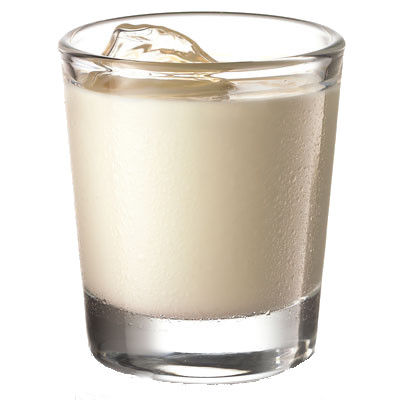
\includegraphics[width=5.5cm]{img/vasito.jpg}}
\tableofcontents\newpage

\section{Data structures}
\subsection{Segment tree}
\cppfile{data_structures/segment_tree.cpp}
\subsection{Segment tree - Lazy propagation}
\cppfile{data_structures/segment_tree_lazy.cpp}
\subsection{Segment tree - Persistence}
\cppfile{data_structures/segment_tree_persistent.cpp}
\subsection{Segment tree - 2D}
\cppfile{data_structures/segment_tree_2d.cpp}
\subsection{Sparse table (static RMQ)}
\cppfile{data_structures/sparse_table.cpp}
\subsection{Fenwick tree}
\cppfile{data_structures/fenwick_tree.cpp}
\subsection{Wavelet tree}
\cppfile{data_structures/wavelet_tree.cpp}
\subsection{STL extended set}
\cppfile{data_structures/stl_extended_set.cpp}
\subsection{STL rope}
\cppfile{data_structures/stl_rope.cpp}
\subsection{Treap (as BST)}
\cppfile{data_structures/treap.cpp}
\subsection{Treap (implicit key)}
\cppfile{data_structures/treap_implicit.cpp}
\subsection{Link-Cut tree}
\cppfile{data_structures/link_cut_tree.cpp}
\subsection{Convex hull trick (static)}
\cppfile{data_structures/convexhull_trick.cpp}
\subsection{Convex hull trick (dynamic)}
\cppfile{data_structures/convexhull_trick_dynamic.cpp}
\subsection{Gain-cost-set}
\cppfile{data_structures/gain_cost_set.cpp}
\subsection{Disjoint intervals}
\cppfile{data_structures/disjoint_intervals.cpp}

\section{Graphs}
\subsection{Topological sort}
\cppfile{graphs/toposort.cpp}
\subsection{Kruskal (+ Union-Find)}
\cppfile{graphs/kruskal.cpp}
\subsection{Dijkstra}
\cppfile{graphs/dijkstra.cpp}
\subsection{Bellman-Ford}
\cppfile{graphs/bellman_ford.cpp}
\subsection{Floyd-Warshall}
\cppfile{graphs/floyd_warshall.cpp}
\subsection{Strongly connected components (+ 2-SAT)}
\cppfile{graphs/tarjan_2sat.cpp}
\subsection{Articulation - Bridges - Biconnected}
\cppfile{graphs/articulation_bridges_biconnected.cpp}
\subsection{Chu-Liu (minimum spanning arborescence)}
\cppfile{graphs/chu_liu.cpp}
\subsection{LCA - Binary Lifting}
\cppfile{graphs/lca.cpp}
\subsection{Heavy-Light decomposition}
\cppfile{graphs/hld.cpp}
\subsection{Centroid decomposition}
\cppfile{graphs/centroid.cpp}
\subsection{Parallel DFS}
\cppfile{graphs/parallel_dfs.cpp}
\subsection{Eulerian path}
\cppfile{graphs/eulerian_path.cpp}
\subsection{Dynamic connectivity}
\cppfile{graphs/dynamic_connectivity.cpp}

\section{Math}
\subsection{Identities}
{
$C_n = \frac{2(2n-1)}{n+1} C_{n-1}$

$C_n = \frac{1}{n+1} \binom{2n}{n}$

$C_n \sim \frac{4^n}{n^{3/2}\sqrt{\pi}}$

$\sigma(n) = O(\log(\log(n)))$ (number of divisors of $n$)

$F_{2n+1} = F_{n}^2 + F_{n+1}^2$

$F_{2n} = F_{n+1}^2 - F_{n-1}^2$

$\sum_{i=1}^n F_i = F_{n+2}-1$

$F_{n+i}F_{n+j} - F_nF_{n+i+j} = (-1)^n F_iF_j$

(Möbius Inv. Formula)
Let $g(n) = \sum_{d\mid n} f(d)$, then $f(n)=\sum{d\mid n} g(d) \mu\left(\frac{n}{d})\right)$.
}
\subsection{Theorems}
\cppfile{math/theorems.txt}
\subsection{Integer floor division}
\cppfile{math/floor_division.cpp}
%\subsection{Extended Euclid} % allready in diophantine
%\cppfile{math/extended_euclid.cpp}
\subsection{Sieve of Eratosthenes}
\cppfile{math/sieve.cpp}
\subsection{Generate divisors}
\cppfile{math/divisors.cpp}
\subsection{Pollard's rho}
\cppfile{math/pollard_rho.cpp}
\subsection{Simpson's rule}
\cppfile{math/simpson.cpp}
\subsection{Polynomials}
\cppfile{math/polynomial.cpp}
\subsection{Bairstow}
\cppfile{math/bairstow.cpp}
\subsection{Fast Fourier Transform}
\cppfile{math/fft.cpp}
\subsection{Karatsuba}
\cppfile{math/karatsuba.cpp}
\subsection{Diophantine}
\cppfile{math/diophantine.cpp}
\subsection{Mobius}
\cppfile{math/mobius.cpp}
\subsection{Modular inverse}
\cppfile{math/inversemod.cpp}
\subsection{Matrix operations}
\cppfile{math/matrix.cpp}
\subsection{Simplex}
\cppfile{math/simplex.cpp}

\section{Geometry}
\subsection{Point}
\cppfile{geometry/point.cpp}
\subsection{Line}
\cppfile{geometry/line.cpp}
\subsection{Circle}
\cppfile{geometry/circle.cpp}
\subsection{Area of intersection of circles}
\cppfile{geometry/circle_area_intersection.cpp}
\subsection{Polygon}
\cppfile{geometry/polygon.cpp}
\subsection{Plane}
\cppfile{geometry/plane.cpp}
\subsection{Radial order of points}
\cppfile{geometry/radial_order.cpp}
\subsection{Convex hull}
\cppfile{geometry/convex_hull.cpp}
\subsection{Dual from planar graph}
\cppfile{geometry/planar_graph_dual.cpp}

\section{Strings}
\subsection{KMP}
\cppfile{strings/kmp.cpp}
\subsection{Z function}
\cppfile{strings/z_function.cpp}
\subsection{Manacher}
\cppfile{strings/manacher.cpp}
\subsection{Aho-Corasick}
\cppfile{strings/aho_corasick.cpp}
\subsection{Suffix automaton}
\cppfile{strings/suffix_automaton.cpp}
%\subsection{Suffix array (shorter but slower)}
%\cppfile{strings/suffix_array_slow.cpp}
\subsection{Suffix array}
\cppfile{strings/suffix_array.cpp}
\subsection{LCP (Longest Common Prefix)}
\cppfile{strings/lcp.cpp}
\subsection{Hashing}
\cppfile{strings/hashing.cpp}
\subsection{Hashing with ll (using \_\_int128)}
\cppfile{strings/hashing_128.cpp}

\section{Flow}
\subsection{Matching (slower)}
\cppfile{flow/matching.cpp}
\subsection{Matching (Hopcroft-Karp)}
\cppfile{flow/hopcroft_karp.cpp}
\subsection{Hungarian}
\cppfile{flow/hungarian.cpp}
\subsection{Dinic}
\cppfile{flow/dinic.cpp}
\subsection{Min cost max flow}
\cppfile{flow/min_cost_max_flow.cpp}

\section{Other}
\subsection{Mo's algorithm}
\cppfile{other/mos_algorithm.cpp}
\subsection{Divide and conquer DP optimization}
\cppfile{other/divide_and_conquer_dp.cpp}
\subsection{Dates}
\cppfile{other/dates.cpp}
\subsection{C++ stuff}
\cppfile{other/cpp_stuff.cpp}
\subsection{Interactive problem tester template}
\cppfile{other/interactive_tester.py}
\subsection{Max number of divisors up to 10\textsuperscript{n}}
\cppfile{other/hcn.txt}

\end{document}
